%----------------------------------------------------------------------------------
% Exemplo do uso da classe tcc.cls. Veja o arquivo .cls
% para mais detalhes e instruções.
%----------------------------------------------------------------------------------

%[ ] Literature Review: the literature review is meant to convey your knowledge of the subject matter of the proposal, so check for
    %[ ] Does it provide basic definitions of the area?
    %[ ] Terminology dropping from the sky: new technical terms must be explained before they are used, avoid talk about a deteronic frombotzer if you have not said what this is
    %[ ] Consistency of terminology: do not use different terms to refer to the same technical entity, once you define something as X always refer to it as X
    %[ ] Are the references up to date: i.e. do you cite work that was published in the last 5-10 years


\chapter{Fundamentação Teórica}\label{chap2:fund_teo}
    
    \section{Veículo de Superfície Não Tripulado}\label{subchap2:USV}
        Um veículo de superfície não tripulado (do inglês \textit{"Unmanned Surface Vehicle"} - USV) é caracterizado por realizar atividades navais de forma autônoma, ou controlado remotamente, sem a presença de tripulação~\cite{LIU201671}. Tais características também enquadram um USV na categoria de um robô~\cite{JURAK2020}.
        De acordo com Liu \etal~\cite{LIU201671}, um USV pode ter as mais variadas aparências e funcionalidades, porém os seguintes componentes básicos devem compor um USV:
        
        \begin{enumerate}
            \item Casco e estruturas mecânicas auxiliares
            \item Sistema de Propulsão
            \item Sistema GNC (\textit{"Guidance Navigation and Control"})
            \item Sistema de Comunicação
            \item Equipamento de Coleta de Dados
            \item Estação de Solo
        \end{enumerate}
        
        Dentre os elementos listados o sistema GNC é fundamental para automatizar um USV, pois ele controlará o sistema do USV como um todo. Sua função consiste coletar informações a respeito do USV e seu entorno (\textit{"Navigation"}), gerenciar dados de missão encontrando o caminho necessário para completá-la (\textit{"Guidance"}) e executar as ações necessárias para atingir o objetivo desejado (\textit{"Control"})~\cite{LIU201671}.
        
        \begin{figure}
            \centering
            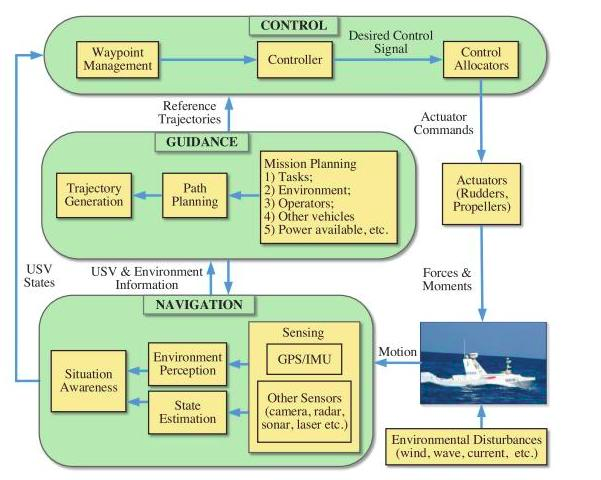
\includegraphics[width=\textwidth]{fig/chap2/gnc_system.png}
            \caption{Caption}
            \label{fig:Liu2016_gncSystem}
        \end{figure}
    
        A Figura ~\ref{fig:Liu2016_gncSystem} apresentada por Liu \etal~\cite{LIU201671} mostra o sistema GNC em detalhe apontando suas funções. Tais funções serão brevemente explicadas a seguir.
        
        \begin{enumerate}
            \item \textit{"Navigation":} subsistema responsável pela coleta de informações a respeito do barco (posição, velocidade, etc) e seu entorno (obstáculos estáticos e obstáculos móveis). Essas informações são coletadas por meio de sensores, radares, câmeras, cartas náuticas e mapas. Os dados coletados são enviados para o subsistema \textit{"Guidance"} e de \textit{"Control"}~\cite{JURAK2020}.
            
            \item \textit{"Guidance":} subsistema responsável por gerenciar os dados da missão atual a ser executada e definir os meios necessários para cumpri-la. Através dos dados obtidos do subsistema \textit{"Navigation"}, as ações necessárias para atingir o objetivo são definidas e enviadas para o subsistema \textit{"Guidance"}~\cite{JURAK2020}.
            
            % As informações referentes ao próprio barco captadas pelo sistema de navegação também vão para o sistema de controle, pois ele precisa saber a posição atual do barco para saber como ele vai atuar para chegar na próxima posição determinada pelo guidance
            \item \textit{"Control":} subsistema que, com base no estado atual do USV obtido pelo subsistema \textit{"Navigation"}, gera os comandos necessários para realizar as ações definidas pelo subsistema \textit{"Guidance"}. Além disso, também é sua responsabilidade executar os comandos gerados diretamente nos atuadores do USV~\cite{JURAK2020}.
        \end{enumerate}
        
        Visto que este trabalho almeja aprimorar a capacidade de evasão de colisão, focaremos no subsistema de \textit{"Guidance"}. Sua implementação consiste em, além do gerenciamento dos dados de missão, estabelecer qual a melhor rota para o USV percorrer~\cite{JURAK2020}. A definição da rota geralmente ocorre em dois níveis: global e local. Ambos os níveis utilizam planejadores; o planejador global definirá a rota a ser corrida em um mapa de larga escala, chamada de rota global, considerando obstáculos estáticos conhecidos; enquanto que o planejador local atentará para o surgimento de obstáculos que não foram considerados na rota global e que precisarão ser desviados, gerando uma rota local específica para a atual situação~\cite{LIU201671}.
    
    \section{Regulamentos Internacionais para Prevenção de Colisões no Mar}\label{subchap2:colregs}
        Buscando padronizar as ações tomadas para evitar colisões, a Organização Internacional da Marinha (IMO - do inglês \textit{"International Marine Organization"}) definiu uma série de regulamentações para colisão no mar (COLREGS - do inglês \textit{"COLlision REGulations at Sea"})~\cite{COLREGS}.
        Para que o uso de USV não apresente perigo para outras embarcações, sendo elas triupuladas ou não, é necessário que ele não realize ações inesperadas pela embarcação que se aproxima. Sendo assim, o USV deverá realizar suas ações de acordo com a COLREGS de forma que seja perceptível para o humano que estiver no outro barco~\cite{KUWATA2014110}.
        
        Jurak~\cite{JURAK2020} em seu sistema considerou os encontros \textit{"head-on"}, \textit{"crossing from left"}, \textit{"crossing from right"} e \textit{"overtaking"}. As situações listadas são ilustradas na Figura~\ref{fig:Jurak2020_colregsSituations} e serão explicados a seguir: 
        
        \begin{figure}
            \centering
            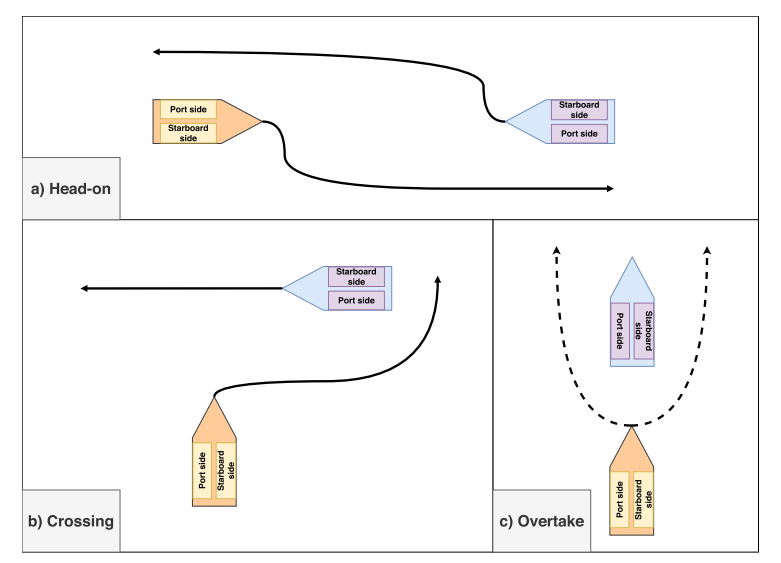
\includegraphics[width=\textwidth]{fig/chap2/colregs_situations.png}
            \caption{Caption}
            \label{fig:Jurak2020_colregsSituations}
        \end{figure}
        
        \begin{enumerate}
            \item [1] \textit{"head-on":} situação em que as embarcações se encontram frente a frente. Nesse caso, a COLREGS especifíca que ambas as embarcações devem evitar a colisão virando à \textit{"starboard side"} (estibordo) e, por consequência, passando pelo \textit{"port side"} (bombordo) do outro navio.
            
            \item [2] \textit{"crossing from left/right":} situação em que uma embarcação cruzará o caminho da outra. Nesse caso, a embarcação que possuir a outra no seu lado direito (\textit{"startboard side"} - estibordo) é responsável por evitar a colisão contornando a embarcação que se aproxima por trás, realizando uma conversão à direita (\textit{"startboard"} - estibordo). Já a embarcação que possuir a outra no seu lado esquerdo (\textit{"port side"} - bombordo), não deverá mudar seu curso.
            
            \item [3] \textit{"overtaking":} situação em que uma embarcação se encontra em uma velocidade maior do que a embarcação que se encontra à frente. Nesse caso a embarcação que se aproxima pode desviar pelo lado em que não causará uma nova situação de \textit{"overtaking"}.
        \end{enumerate}
    
    \section{Evasão de Colisão}\label{subchap2:prev_col}
        %Falar aqui, de alguma forma, que evasão de colisão se refere a "se" e "quando" agir frente a uma possível colisão
        Uma tarefa primordial quando se trata de navegação é evitar que a embarcação colida com algum obstáculo. Entretanto, prevenção de colisão consiste em um dos principais desafios ao desenvolver um USV~\cite{JURAK2020}. Em um USV o sistema GNC é responsável por realizar todo o procedimento de prevenção de colisão, sendo o subsistema \textit{"Guidance"} o encarregado de detectar a colisão e encontrar uma solução para que ela não ocorra~\cite{HUANG2020451}.
        
        Huang \etal (2020, p.451) define prevenção de colisão como:
        \begin{directcite}
            \textit{"Prevenção de colisão é o processo em que um navio desvia de sua trajetória planejada para evitar contato físico indesejado em um certo tempo futuro"}
        \end{directcite}
        
        Com isso, Huang \etal~\cite{HUANG2020451} separa o processo de prevenção de colisão nas seguintes etapas: 
        
        \begin{enumerate}
            \item Previsão de Movimento: que prevê estados futuros do OS e dos TSs envolvidos;
            \item Detecção de Conflito: determina se o OS está em risco de colisão;
            \item Resolução de Conflito: encontrará o melhor caminho para evitar a colisão.
        \end{enumerate}
        
        A Figura~\ref{fig:Huang2020_collisionAvoidanceProcess}, apresentada por Huang \etal~\cite{HUANG2020451}, mostra o fluxo de informação realizada em um sistema GNC no procedimento de prevenção de colisão. Na imagem, podemos considerar \textit{"Observer"} e \textit{"Actuator"} como módulos dos subsistemas de \textit{"Navigation"} e \textit{"Control"}, respectivamente. Os módulos envoltos pelo pontilhado vermelho correspondem às etapas listadas anteriormente e que compõe o subsistema \textit{"Guidance"}.
        
        As informações coletadas pelo \textit{"Observer"} são utilizadas pelo módulo \textit{"Motion Prediction"}, quando implementado, para realizar as previsões necessárias. O módulo \textit{"Conflict Detection"} utilizará as informações providas pelo \textit{"Motion Prediction"}, ou \textit{"Observer"}, a fim de identificar se há risco de colisão. Se não houver, as diretivas de caminho e velocidade são enviadas diretamente para o \textit{"Actuator"}. Caso houver risco de colisão, o módulo \textit{"Conflict Resolution"} será acionado para que encontre um caminho seguro para evitar a colisão, consequentemente, gerando diretivas de caminho e velocidade que levarão a um desvio da rota global.
        
        \begin{figure}
            \centering
            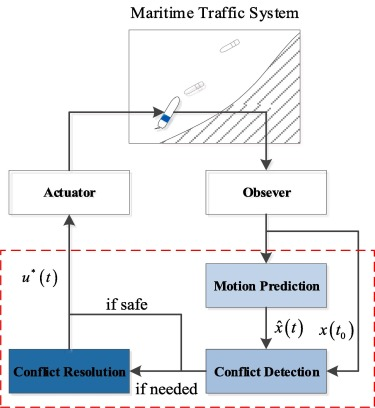
\includegraphics{fig/chap2/information_flow.png}
            \caption{Fluxo de informação ~\cite{HUANG2020451}}
            \label{fig:Huang2020_collisionAvoidanceProcess}
        \end{figure}
        
        Dentre as categorias de métodos de evasão de colisão, sendo eles baseados na vivência de marinheiros experientes ou então em modelos puramente matemáticos~\cite{HUANG2020451}, este trabalho tratará a respeito do primeiro caso. Deste modo, tralharemos com indicadores para avaliar o risco de uma colisão acontecer ou não, comumente chamado na literatura de Índice de Risco de Colisão (do inglês \textit{"Collision Risk Index" - CRI})~\cite{HUANG2019142}.
        
    \section{Ponto de Maior Aproximação}\label{subchap2:cpa}
        Um meio popular de se avaliar o CRI é através do método de CPA. Nele, dois índices são considerados: Distância para o Ponto de maior Aproximação (do inglês \textit{"Distance to Closest Point of Approach"} - DCPA), e Tempo para o Ponto de Maior Aproximação (do inglês \textit{"Time to Closest Point of Approach"} - TCPA)~\cite{HUANG2019142}. Ambos índices são valores numéricos e contribuem para um maior, ou menor, CRI, que também é um valor numérico. Quando o valor resultante é superior a um limite (\textit{threshold}), é detectado um risco de colisão eminente e o procedimento para evitar o acidente é iniciado~\cite{HUANG2020451}. 
        
        Tais indicadores poderiam ser obtidos através da predição da posição dos navios para cada instante de tempo futuro. Porém esse processamento deveria ser reexecutado a todo momento pelo GNC, demandando um grande esforço computacional. Em contrapartida, utilizando o algoritimo de Obstáculo de Velocidades (do inglês \textit{"Velocity Obstacles"} - VO) é possível identificar uma situação de colisão em qualquer tempo futuro com apenas uma verificação, simplificando o problema para um de primeira ordem~\cite{KUWATA2014110}. Além disso, outra vantagem de utilizar VO é que esse algoritmo escala de forma satisfatória para encontros com múltiplos obstáculos móveis. Contudo, o principal desafio no uso de VO consiste em faze-lo considerar a dinâmica do barco, ou seja, não assumir que poderá alterar sua velocidade linear ou angular instantaneamente~\cite{HUANG2019142}.
        
    \section{Obstáculos de Velocidade}\label{subchap2:vo}
        O algoritmo VO consiste em identificar um conjunto de velocidades que conduzirão o USV por um caminho livre de colisão~\cite{HUANG2019142}. Isso é feito gerando um obstáculo no espaço de velocidades com a garantia que, enquanto o vetor velocidade do USV estiver fora do obstáculo gerado, não haverá colisão em qualquer tempo futuro. Esse obstáculo possui um formato cônico com suas arestas tangenciando o TS expandido pelo tamanho do USV~\cite{KUWATA2014110}. Essa expansão também pode ser representada por um círculo como apresentado por Song \etal~\cite{SONG2018351}.
        
        Neste trabalho adaptaremos o algoritmo de VO apresentado por Kuwata \etal ~\cite{KUWATA2014110} para que seja integrado no sistema desenvolvido por Jurak~\cite{JURAK2020}. Para tal, é preciso introduzir as notações utilizadas pelo autor em seu trabalho. Sendo assim, consideraremos o vetor $\vec{p} \in \R^2$ como sendo a posição da embarcação e o vetor $\vec{v} \in \R^2$ a sua velocidade. Kuwata \etal ~\cite{KUWATA2014110} ainda define as seguintes equações para obter o vetor velocidade partindo de $\vec{p}$ (equação \eqref{subchap2:eqVelocityVector}) e a expansão da área ocupada pelo obstáculo (equação \eqref{subchap2:eqMinkowskiSum} e \eqref{subchap2:eqReflection}):
        % comentário para evitar novo parágrafo
        \begin{align}
            \text{Vetor velocidade de $\vec{p}$ até $\vec{v}$:}\quad&~\lambda(\vec{p}, \vec{v}) = \{\vec{p} + t\vec{v}~|~t \geq 0\}\label{subchap2:eqVelocityVector}\\
            \text{Soma de Minkowski:}\quad&~\mathcal{A} \oplus \mathcal{B}= \{\vec{a} + \vec{b}~|~\vec{a} \in \mathcal{A}, \vec{b} \in \mathcal{B}\}\label{subchap2:eqMinkowskiSum}\\
            \text{Reflexão:}\quad&~- \mathcal{A}= \{- \vec{a}~|~\vec{a} \in \mathcal{A}\}\label{subchap2:eqReflection}
        \end{align}
        
        \begin{figure}
            \centering
            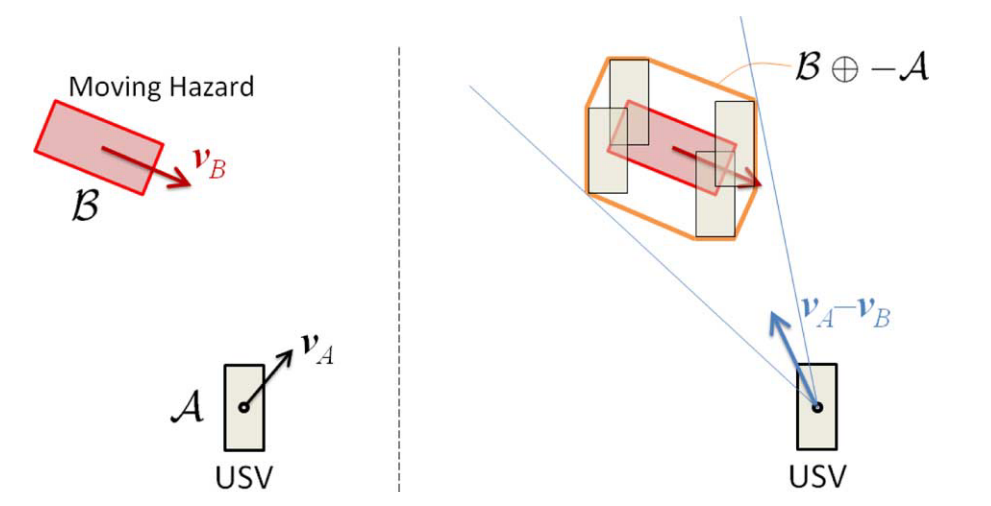
\includegraphics[width=\textwidth]{fig/chap2/vo.png}
            \caption{Caption}
            \label{fig:Kuwata2014_vo}
        \end{figure}
       % Considerando a situação da Figura~\ref{fig:Kuwata2014_vo}, apresentada por Kuwata \etal~\cite{KUWATA2014110}, temos, no lado esquerdo, que um dado USV $\mathcal{A}$ se move a uma velocidade $\vec{v_\mathcal{A}}$ enquanto que um obstáculo em movimento $\mathcal{B}$ se move a uma velocidade $\vec{v_\mathcal{B}}$. O VO gerado por $\mathcal{B}$ no espaço de velocidade de $\mathcal{A}$ é mostrado no lado direito da imagem e definido pela equação \eqref{eq:velocityObstacle}. Neste primeiro momento, com o vértice do VO no centro do USV, temos que a colisão é identificada dado que o vetor resultate de $(\vec{v_\mathcal{A}} - \vec{v_\mathcal{B}})$ esta direcionado para o interior do VO. 
        Considerando a situação da Figura~\ref{fig:Kuwata2014_vo}, apresentada por Kuwata \etal~\cite{KUWATA2014110}, temos, no lado esquerdo, que um dado USV $\mathcal{A}$ se move a uma velocidade $\vec{v_\mathcal{A}}$ enquanto que um obstáculo em movimento $\mathcal{B}$ se move a uma velocidade $\vec{v_\mathcal{B}}$. Como o vetor resultante da operação $(\vec{v_\mathcal{A}} - \vec{v_\mathcal{B}})$ aponta em direção ao obstáculo $\mathcal{B}$ expandido pelo tamanho de $\mathcal{A}$, haverá colisão. O VO gerado por $\mathcal{B}$ no espaço de velocidade de $\mathcal{A}$ é o mesmo cone mostrado na figura, porém deslocado por $\mathcal{B}$. Sua definição é dada por:
        % Comentário para evitar novo parágrafo
        \begin{equation}\label{eq:velocityObstacle}
            \mathcal{VO^A_B}(\vec{v_\mathcal{B}}) = \{\vec{v_\mathcal{A}}~|~\lambda(\vec{p_\mathcal{A}}, \vec{v_\mathcal{A}} - \vec{v_\mathcal{B}}) \cap (\mathcal{B} \oplus \mathcal{A}) \neq \varnothing\}
        \end{equation}